\section{The Pattern family}

Let's try something different now. Type and run this line of code:

\begin{lstlisting}[style=SuperCollider-IDE, basicstyle=\scttfamily\footnotesize]
Pbind(\degree, Pseries(0, 1, 30), \dur, 0.05).play;
\end{lstlisting}

\subsection{Meet Pbind}

\texttt{Pbind} is a member of the Pattern family in SuperCollider. The capital P in \texttt{Pbind} and \texttt{Pseries} stands for \emph{Pattern}; we'll meet other members of the family soon. For now, let's take a closer look at \texttt{Pbind} only. Try this stripped down example:

\begin{lstlisting}[style=SuperCollider-IDE, basicstyle=\scttfamily\footnotesize]
Pbind(\degree, 0).play;
\end{lstlisting}

The only thing this line of code does in life is to play the note \emph{middle C}, one time per second. The keyword \texttt{\textbackslash degree} refers to scale degrees, and the number 0 means the first scale degree (a C major scale is assumed, so that's the note C itself). Note that SuperCollider starts counting things from 0, not from 1. In a simple line like the above, the notes C, D, E, F, G\dots would be represented by the numbers 0, 1, 2, 3, 4\dots Try changing the number and notice how the note changes when you re-evaluate. You can also choose notes below middle C by using negative numbers (for example, -2 will give you the note A below middle C). In short, just imagine that the middle C note of the piano is 0, and then count white keys up or down (positive or negative numbers) to get any other note.

Now play around a bit with the duration of the notes. \texttt{Pbind} uses the keyword \texttt{\textbackslash dur} to specify durations in seconds:

\begin{lstlisting}[style=SuperCollider-IDE, basicstyle=\scttfamily\footnotesize]
Pbind(\degree, 0, \dur, 0.5).play;
\end{lstlisting}

Of course this is still very rigid and inflexible---always the same note, always the same duration. Don't worry: things will get better very soon. But first let's take a look at the other ways you can specify pitch inside a Pbind.

\subsection{Pseq}

Let's go ahead and play several notes in sequence, like a scale. Let's also make our notes shorter, say, 0.2 second long.
 
\begin{lstlisting}[style=SuperCollider-IDE, basicstyle=\scttfamily\footnotesize]
Pbind(\degree, Pseq([0, 1, 2, 3, 4, 5, 6, 7], 1), \dur, 0.2).play;
\end{lstlisting}

This line introduces a new member of the Pattern family: \texttt{Pseq}. As the name might suggest, this pattern deals with sequences. All that \texttt{Pseq} needs in order to play a sequence is:
\begin{itemize}
\item a list of items between square brackets
\item a number of repetitions.
\end{itemize} 

In the example, the list is \texttt{[0, 1, 2, 3, 4, 5, 6, 7]}, and the number of repeats is \texttt{1}. This \texttt{Pseq} simply means: ``play once all the items of the list, in sequence.'' Notice that these two elements, list and number of repeats, are inside \texttt{Pseq}'s own parentheses, and they are separated by a comma.

Also notice where \texttt{Pseq} appears within the \texttt{Pbind}: it is the input value of \texttt{\textbackslash degree}. This is important: instead of providing a single, fixed number for scale degree (as in our first simple \texttt{Pbind}), \emph{we are providing a whole Pseq: a recipe for a sequence of numbers}. With this in mind, we can easily expand upon this idea and use another Pseq to control durations as well:

 
\begin{lstlisting}[style=SuperCollider-IDE, basicstyle=\scttfamily\footnotesize]
Pbind(\degree, Pseq([0, 1, 2, 3, 4, 5, 6, 7], 5), \dur, Pseq([0.2, 0.1, 0.1, 0.2, 0.2, 0.35], inf)).play;
\end{lstlisting}
 
What is happening in this example? First, we have changed the number of repeats of the first \texttt{Pseq} to 5, so the entire scale will play five times. Second, we have replaced the previously fixed \texttt{\textbackslash dur} value of 0.2 with another \texttt{Pseq}. This new \texttt{Pseq} has a list of six items: \texttt{[0.2, 0.1, 0.1, 0.2, 0.2, 0.35]}. These numbers become duration values for the resulting notes. The \texttt{repeats} value of this second \texttt{Pseq} is set to \texttt{inf}, which stands for ``infinite.'' This means that the \texttt{Pseq} has no limit on the number of times it can repeat its sequence. Does the \texttt{Pbind} play forever, then? No: it stops after the \emph{other} \texttt{Pseq} has finished its job, that is, after the sequence of scale degrees has been played 5 times.

Finally, the example has a total of eight different notes (the list in the first \texttt{Pseq}), while there are only six values for duration (second \texttt{Pseq}). When you provide sequences of different sizes like this, \texttt{Pbind} simply cycles through them as needed.

Answer these questions to practice what you have learned:
\begin{itemize}
\item Try the number 1 instead of inf as the \texttt{repeats} argument of the second \texttt{Pseq}. What happens?
\item How can you make this Pbind play forever?
\end{itemize}

Solutions are at the end of the book.\endnote{First question: when you use the number 1 instead of \texttt{inf} as the \texttt{repeats} argument of the second \texttt{Pseq}, the Pbind will stop after 6 notes have been played (that is, after one full sequence of duration values has been performed). Second question: to make a Pbind play forever, simply use \texttt{inf} as the \texttt{repeats} value of all inner patterns.}

\subsection{Make your code more readable}

You may have noticed that the line of code above is quite long. In fact, it is so long that it wraps to a new line, even though it is technically a single statement. Long lines of code can be confusing to read. To avoid this, it is common practice to break the code into several indented lines; the goal is to make it as clear and intelligible as possible. The same \texttt{Pbind} above can be written like this:

\begin{lstlisting}[style=SuperCollider-IDE, basicstyle=\scttfamily\footnotesize]
(
Pbind(
	\degree, Pseq([0, 1, 2, 3, 4, 5, 6, 7], 5),
	\dur, Pseq([0.2, 0.1, 0.1, 0.2, 0.2, 0.35], inf)
).play;
)
\end{lstlisting}

From now on, get into the habit of writing your \texttt{Pbind}s like this. Writing code that looks neatly arranged and well organized will help you a lot in learning SuperCollider.

Also, notice that we enclosed this \texttt{Pbind} within parentheses to create a code block (remember section \ref{sec:code-block}?): because it is no longer in a single line, we need to do this to be able to run it all together. Just make sure the cursor is anywhere within the block before evaluating.


\subsection{Four ways of specifying pitch}

\texttt{Pbind} accepts other ways of specifying pitch, not just scale degrees.
\begin{itemize}
\item If you want to use all twelve chromatic notes (black and white keys of the piano), you can use \texttt{\textbackslash note} instead of \texttt{\textbackslash degree}. 0 will still mean middle C, but now the steps include black keys of the piano (0=middle C, 1=C$\sharp$, 2=D, etc).
\item  If you prefer to use MIDI note numbering, use \texttt{\textbackslash midinote} (60=middle C, 61=C$\sharp$, 62=D, etc).
\item Finally, if you'd rather specify frequencies directly in Herz, use \texttt{\textbackslash freq}.
\end{itemize}

See Figure \ref{fig:scale-degrees} for a comparison of all four methods.

\begin{figure}[h]
\centering
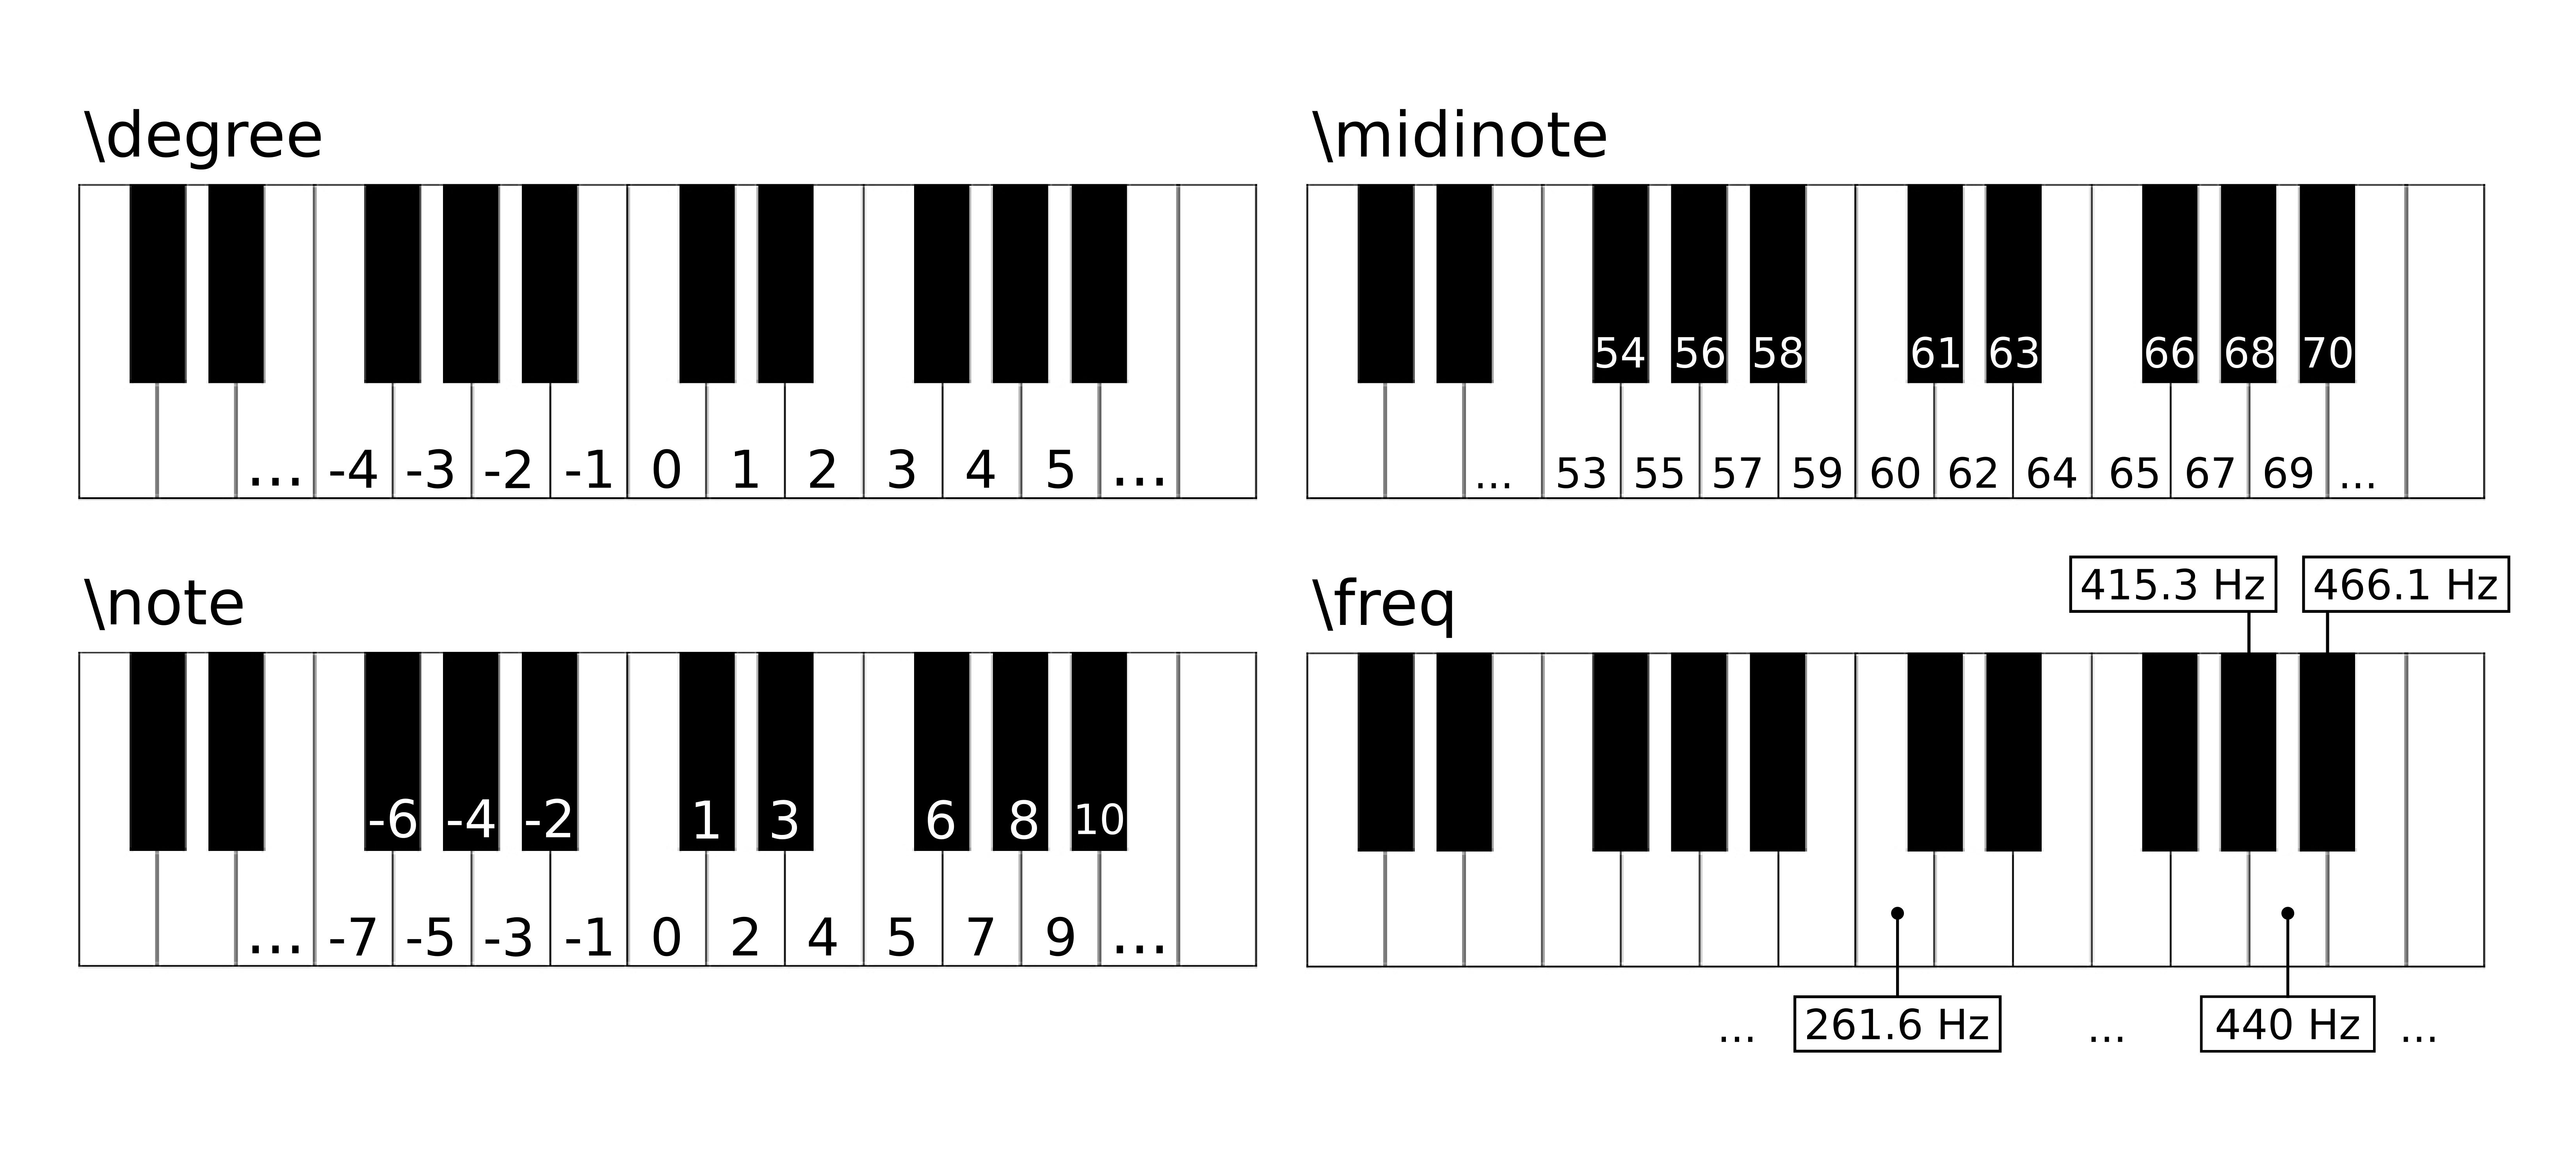
\includegraphics[scale=0.4]{fig-piano-keyboard-degree-note-midinote-freq.png}
\caption{Comparing scale degrees, note numbers, midinotes, and frequencies}
\label{fig:scale-degrees}
\end{figure}

In the next example, the four Pbinds all play the same note: the A above middle C (A4).

\begin{lstlisting}[style=SuperCollider-IDE, basicstyle=\scttfamily\footnotesize]
Pbind(\degree, 5).play;
Pbind(\note, 9).play;
Pbind(\midinote, 69).play;
Pbind(\freq, 440).play;
\end{lstlisting}


\bigskip
\todo[inline, color=green!40]{ 
TIP: Remember that each type of pitch specification expects numbers in a different sensible range. A list of numbers like \texttt{[-1, 0, 1, 3]} makes sense for \texttt{\textbackslash degree} and \texttt{\textbackslash note}, but doesn't make sense for \texttt{\textbackslash midinote} nor \texttt{\textbackslash freq}. The table below compares some values using the piano keyboard as a reference.
}
\bigskip


\begin{tabular}{|l|c|c|c|c|c|}
\hline 
  & \textbf{A0 (lowest piano note)} & \textbf{C4} & \textbf{A4} & \textbf{C5} & \textbf{C8 (highest piano note)} \\ 
\hline 
\texttt{\textbackslash degree} & -23 & 0 & 5 & 7 & 21 \\
\hline
\texttt{\textbackslash note} & -39 & 0 & 9 & 12 & 48 \\
\hline
\texttt{\textbackslash midinote} & 21 & 60 & 69 & 72 & 108 \\
\hline
\texttt{\textbackslash freq} & 27.5 & 261.6 & 440 & 523.2 & 4186 \\
\hline
\end{tabular}
\bigskip


\subsection{More keywords: amplitude and legato}

The next example introduces two new keywords: \texttt{\textbackslash amp} and \texttt{\textbackslash legato}, which define the amplitude of events, and the amount of legato between notes. Notice how the code is fairly easy to read thanks to nice indentation and spread over multiple lines. Enclosing parentheses (top and bottom) are used to delimit a code block for quick execution.

 
\begin{lstlisting}[style=SuperCollider-IDE, basicstyle=\scttfamily\footnotesize]
(
Pbind(
	\degree, Pseq([0, -1, 2, -3, 4, -3, 7, 11, 4, 2, 0, -3], 5),
	\dur, Pseq([0.2, 0.1, 0.1], inf),
	\amp, Pseq([0.7, 0.5, 0.3, 0.2], inf),
	\legato, 0.4
).play;
)
\end{lstlisting}
 

\texttt{Pbind} has many of these pre-defined keywords, and with time you will learn more of them. For now, let's stick to just a few---one for pitch (choose from \texttt{\textbackslash degree}, \texttt{\textbackslash note}, \texttt{\textbackslash midinote}, or \texttt{\textbackslash freq}), one for durations (\texttt{\textbackslash dur}), one for amplitude (\texttt{\textbackslash amp}), and one for legato  (\texttt{\textbackslash legato}). Durations are in beats (in this case, 1 beat per second, which is the default); amplitude should be between 0 and 1 (0 = silence, 1 = very loud); and legato works best with values between 0.1 and 1 (if you are not sure about what legato does, simply try the example above with 0.1, then 0.2, then 0.3, all the way up to 1, and hear the results).

Take the last example as point of departure and create new \texttt{Pbind}s. Change the melody. Come up with new lists of durations and amplitudes. Experiment using \texttt{\textbackslash freq} for pitch. Remember, you can always choose to use a fixed number for any given parameter, if that's what you need. For example, if you want all notes in your melody to be 0.2 seconds long, there is no need to write \texttt{Pseq[0.2, 0.2, 0.2, 0.2\dots}, not even \texttt{Pseq([0.2], inf)}---simply remove the whole \texttt{Pseq} structure and write 0.2 in there.

\subsection{Prand}

\texttt{Prand} is a close cousin of \texttt{Pseq}. It also takes in a list and a number of repeats. But instead of playing through the list in sequence, \texttt{Prand} \emph{picks a random item from the list every time}. Try it:

 
\begin{lstlisting}[style=SuperCollider-IDE, basicstyle=\scttfamily\footnotesize]
(
Pbind(
	\degree, Prand([2, 3, 4, 5, 6], inf),
	\dur, 0.15,
	\amp, 0.2,
	\legato, 0.1
).play;
)
\end{lstlisting}
 

Replace \texttt{Prand} with \texttt{Pseq} and compare the results. Now try using \texttt{Prand} for durations, amplitudes, and legato.

\subsection{Pwhite}

Another popular member of the Pattern family is \texttt{Pwhite}. It is an equal distribution random number generator (the name comes from ``white noise''). For example, \texttt{Pwhite(100, 500)} will get you random numbers between 100 and 500.
 
\begin{lstlisting}[style=SuperCollider-IDE, basicstyle=\scttfamily\footnotesize]
(
Pbind(
	\freq, Pwhite(100, 500),
	\dur, Prand([0.15, 0.25, 0.3], inf),
	\amp, 0.2,
	\legato, 0.3
).trace.play;
)
\end{lstlisting}
 

The example above also shows another helpful trick: the message \texttt{trace} just before \texttt{play}. It prints out in the Post window the values chosen for every event. Very useful for debugging or simply to understand what is going on!

Pay attention to the differences between \texttt{Pwhite} and \texttt{Prand}: even though both have to do with randomness, they take in different arguments, and they do different things. Inside \texttt{Pwhite}'s parentheses you only need to provide a low and a high boundary: \texttt{Pwhite(low, high)}. Random numbers will be chosen from within that range. \texttt{Prand}, on the other hand, takes in a list of items (necessarily between square brackets), and a number of repeats: \texttt{Prand([list, of, items], repeats)}. Random items will be chosen \emph{from the list}.

Play around with both and make sure you fully understand the difference.


\bigskip
\todo[inline, color=green!40]{ 
TIP: A \texttt{Pwhite} with two integer numbers will generate only integers. For example, \texttt{Pwhite(100, 500)} will output numbers like 145, 568, 700, but not 145.6, 450.32, etc. If you want floating point numbers in your output, write \texttt{Pwhite(100, 500.0)}. This is very useful for, say, amplitudes: if you write \texttt{Pwhite(0, 1)} you are only getting 0 or 1, but write \texttt{Pwhite(0, 1.0)} and you will get everything in between.
}
\bigskip
 


Try the following questions to test your new knowledge:

\begin{enumerate}[a)]
\item What is the difference in output between \texttt{Pwhite(0, 10)} and \texttt{Prand([0, 4, 1, 5, 9, 10, 2, 3], inf)}?

\item If you need a stream of integer numbers chosen randomly between 0 and 100, could you use a \texttt{Prand}?

\item What is the difference in output between \texttt{Pwhite(0, 3)} and \texttt{Prand([0, 1, 2, 3], inf)}? What if you write \texttt{Pwhite(0, 3.0)}?

\item  Run the examples below. We use \texttt{\textbackslash note} instead of \texttt{\textbackslash degree} in order to play a C minor scale (which includes black keys). The list \texttt{[0, 2, 3, 5, 7, 8, 11, 12]} has eight numbers in it, corresponding to pitches C, D, E$\flat$, F, G, A$\flat$, B, C, but how many events does each example actually play? Why?

 
\begin{lstlisting}[style=SuperCollider-IDE, basicstyle=\scttfamily\footnotesize]
// Pseq
(
Pbind(
	\note, Pseq([0, 2, 3, 5, 7, 8, 11, 12], 4),
	\dur, 0.15;
).play;
)

// Pseq
(
Pbind(
	\note, Prand([0, 2, 3, 5, 7, 8, 11, 12], 4),
	\dur, 0.15;
).play;
)

// Pwhite
(
Pbind(
	\note, Pseq([0, 2, 3, 5, 7, 8, 11, 12], 4),
	\dur, Pwhite(0.15, 0.5);
).play;
)
\end{lstlisting}

\end{enumerate}


Answers are at the end of this tutorial.\endnote{\\
a) \texttt{Pwhite(0, 10)} will generate any number between 0 and 10. \texttt{Prand([0, 4, 1, 5, 9, 10, 2, 3], inf)} will only pick from the list, which has \emph{some} numbers between 0 and 10, but not all (6, 7, 8 are not there, so they will never occur in this \texttt{Prand}).  \\
b) Technically you could use a \texttt{Prand} if you provide a list with all numbers between 0 and 100, but it makes more sense to use a \texttt{Pwhite} for this task: \texttt{Pwhite(0, 100)}. \\
c) \texttt{Prand([0, 1, 2, 3], inf)} picks items from the list at random. \texttt{Pwhite(0, 3)}  arrives at the same kind of output through different means: it will generate random integer numbers between 0 and 3, which ends up being the same pool of options than the \texttt{Prand} above. However, if you write \texttt{Pwhite(0, 3.0)}, the output is now different: because one of the input arguments of \texttt{Pwhite} is written as a float (3.0), it will now output any floating point number between 1 and 3, like 0.154, 1.0, 1.45, 2.999.
\\
d) The first \texttt{Pbind} plays 32 notes (4 times the sequence of 8 notes). The second \texttt{Pbind} plays only 4 notes: four random choices picked from the list (remember that \texttt{Prand}, unlike \texttt{Pseq}, has no obligation to play all the notes from the list: it will simply pick as many random notes as you tell it to). The third and last \texttt{Pbind} plays 32 notes, like the first.
}

\bigskip
\todo[inline, color=green!40]{ 
TIP: A Pbind stops playing when the shortest internal pattern has finished playing (as determined by the \texttt{repeats} argument of each internal pattern).
}
\bigskip

\subsection{Expanding your Pattern vocabulary}

By now you should be able to write simple \texttt{Pbind}s on your own. You know how to specify pitches, durations, amplitudes, and legato values, and you know how to embed other patterns (\texttt{Pseq}, \texttt{Prand}, \texttt{Pwhite}) to generate interesting parameter changes.

This section will expand your Pattern vocabulary a bit. The examples below introduce six more members of the Pattern family. Try to figure out by yourself what they do. Use the following strategies:
\begin{itemize}
\item Listen the resulting melody; describe and analyze what you hear;
\item Look at the Pattern name: does it suggest something? (for example, \texttt{Pshuf} may remind you of the word ``shuffle'');
\item Look at the arguments (numbers) inside the new Pattern;
\item Use \texttt{.trace.play} as seen earlier to watch the values being printed in the Post window;
\item Finally, confirm your guesses by consulting the Help files (select the name of the pattern and hit [ctrl+D] to open the corresponding Help file).
\end{itemize}

%\lstinputlisting[style=SuperCollider-IDE, basicstyle=\scttfamily\footnotesize]{code-pattern-expand-vocabulary.scd}

\begin{lstlisting}[style=SuperCollider-IDE, basicstyle=\scttfamily\footnotesize]
// Expanding your Pattern vocabulary

// Pser
(
Pbind(
	\note, Pser([0, 2, 3, 5, 7, 8, 11, 12], 11),
	\dur, 0.15;
).play;
)

// Pxrand
// Compare with Prand to hear the difference
(
p = Pbind(
    \note, Pxrand([0, 2, 3, 5, 7, 8, 11, 12], inf),
	\dur, 0.15;
).play;
)

// Pshuf
(
p = Pbind(
    \note, Pshuf([0, 2, 3, 5, 7, 8, 11, 12], 6),
	\dur, 0.15;
).play;
)

// Pslide
// Takes 4 arguments: list, repeats, length, step
(
Pbind(
	\note, Pslide([0, 2, 3, 5, 7, 8, 11, 12], 7, 3, 1),
	\dur, 0.15;
).play;
)

// Pseries
// Takes three arguments: start, step, length
(
Pbind(
    \note, Pseries(0, 2, 15),
	\dur, 0.15;
).play;
)

// Pgeom
// Takes three arguments: start, grow, length
(
Pbind(
	\note, Pseq([0, 2, 3, 5, 7, 8, 11, 12], inf),
	\dur, Pgeom(0.1, 1.1, 25);
).play;
)

// Pn
(
Pbind(
	\note, Pseq([0, Pn(2, 3), 3, Pn(5, 3), 7, Pn(8, 3), 11, 12], 1),
	\dur, 0.15;
).play;
)
\end{lstlisting}
 

Practice using these Patterns---you can do a lot with them. \texttt{Pbind}s are like a recipe for a musical score, with the advantage that you are not limited to writing fixed sequences of notes and rhythms: you can describe processes of ever changing musical parameters (this is sometimes called ``algorithmic composition''). And this is just one aspect of the powerful capabilities of the Pattern family.

In the future, when you feel the need for more pattern objects, the best place to go is James Harkins' ``A Practical Guide to Patterns,'' available in the built-in Help files.\footnote{Also online at \url{http://doc.sccode.org/Tutorials/A-Practical-Guide/PG_01_Introduction.html}}